Ссылка на оригинальный конспект: \url{https://github.com/hse-ds/iad-applied-ds/blob/master/2020/lectures/lecture01-recommender.pdf}
	
	Как понять, что пользователю может понравиться товар? Первый вариант — поискать похожих на него пользователей и посмотреть, что нравится им; также можно поискать товары, похожие на те, которые этот пользователь уже покупал. Методы коллаборативной фильтрации строят рекомендации для пользователя на основе похожестей между пользователями и товарами, которые похожие пользователи выбирают.
	
	Сначала необходимо определить, что пользователи похожи между собой. Для этого считается корреляция Пирсона. 
	
	Далее мы можем посчитать сходство товаров исходя из тех рейтингов, что рассматриваемые два пользователя им поставили. 
	
	Эти формулы определения похожести между пользователями приведены здесь:
	
\begin{figure}[H]
\centering
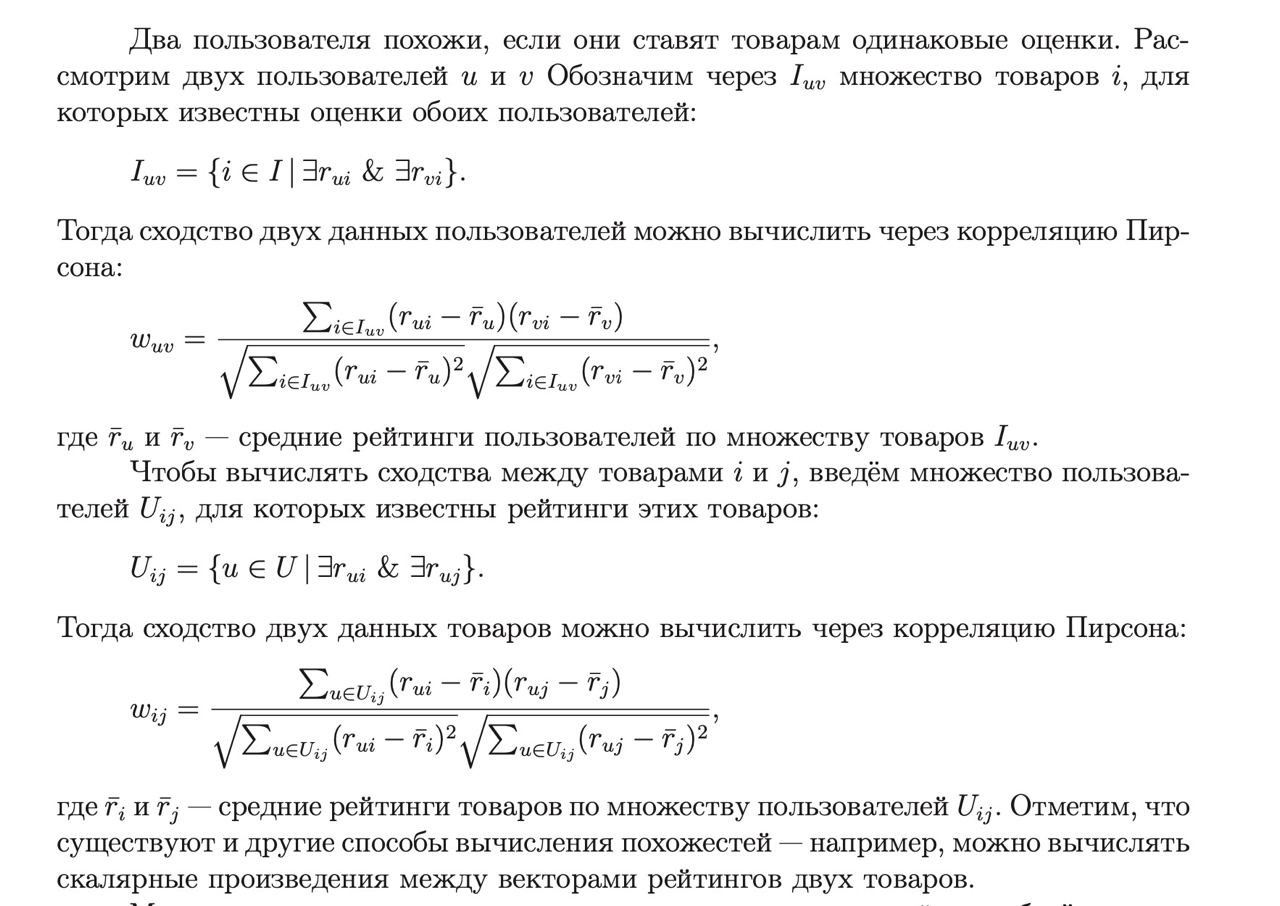
\includegraphics[width=0.7\linewidth]{16_memory1.jpg}
\label{fig:16_memory1} 
\caption{Формулы для определения похожести пользователей}
\end{figure}
	
	
	После того, как мы определили степень похожести товаров между собой и пользователей между собой, нам нужно понять, какие все-таки товары нам рекомендовать пользователю.
	
	Здесь существует два подхода:
	
	1) user-based collaborative filtering 
	
	2) item-based collaborative filtering 
	
	В основе первого подхода лежит процедура, согласно которой мы определяем множество похожих пользователей $U(u_0)$: $U(u_0) = \{v \in U | w_{u_0 v} > \alpha\}$. Эта штука называется коллаборацией, то есть множество похожих пользователей, которые (примерно) одинако оценивают продукты. 
	
	Дальше рекомендуем пользователи те продукты, которые он сам не оценил, но которые хорошо оценили пользователи из коллаборации. 
	
	Для этого мы считаем, как часто товар покупался пользователем из множества $U(u_0) $
		

	
			\begin{figure}[H]
\centering
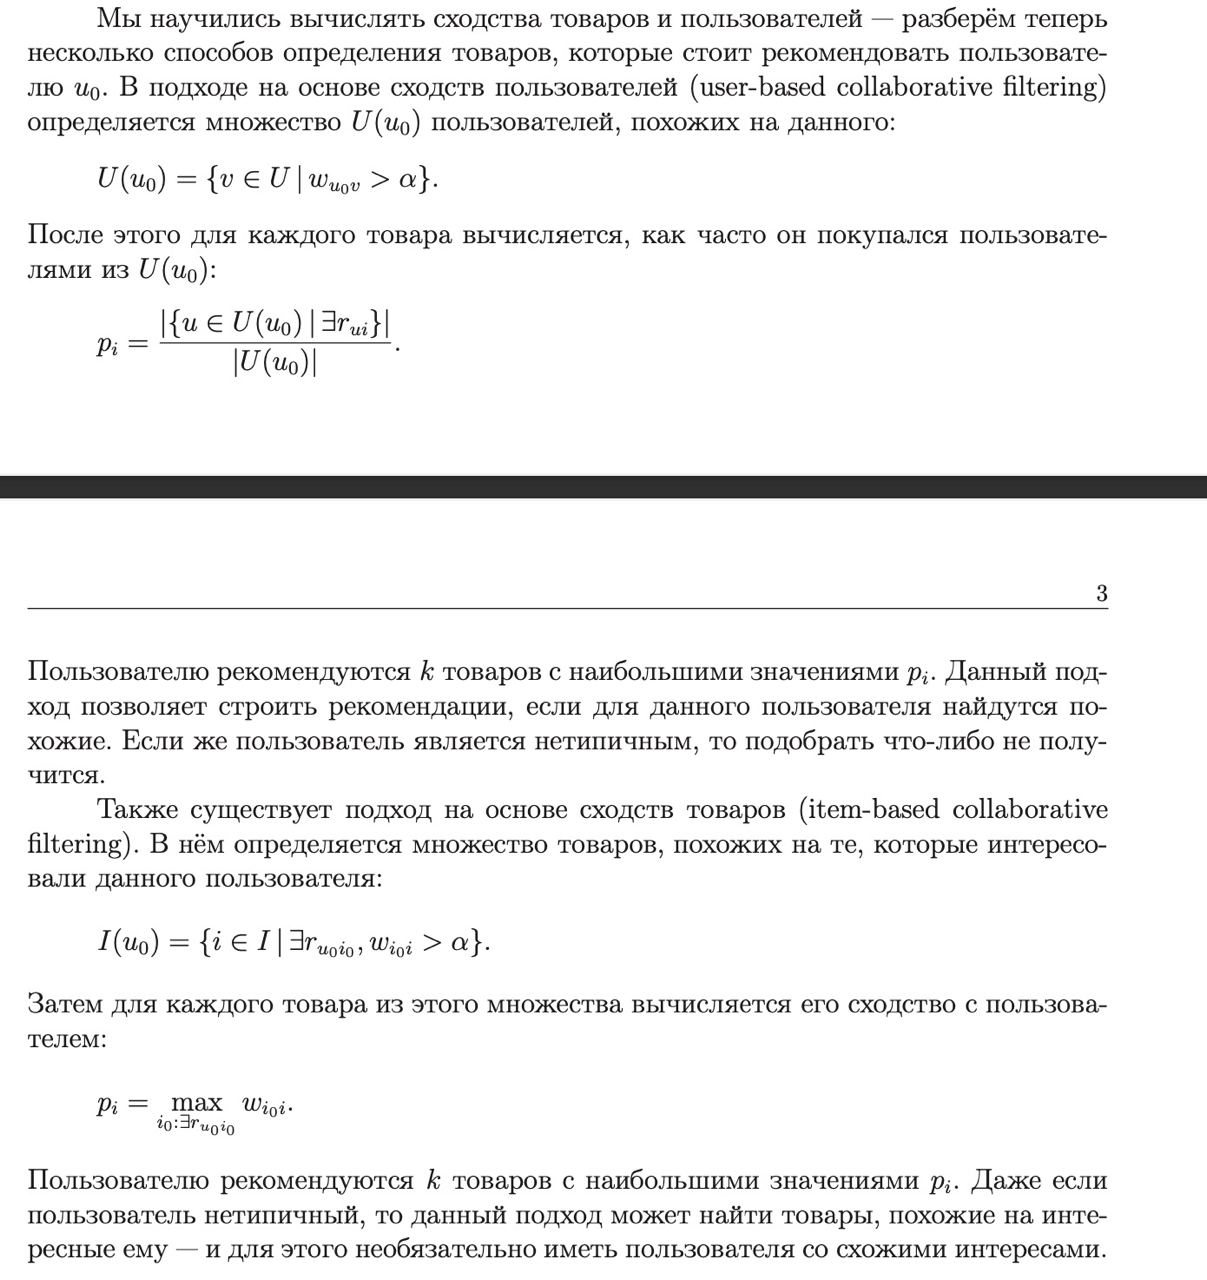
\includegraphics[width=0.7\linewidth]{16_memory2.jpg}
\caption{Формула рассчета частоты покупки товаром пользователями из коллаборации}
\label{fig:16_memory2} 
\end{figure}
